\section{Observational Evidence}
\label{secObservationalEvidence}

The first observation of the presence of invisible matter in the universe has been made in the studies of galactic clusters, in particular during {\it redshift measurements} in the Coma cluster~\cite{RotationCurves_Zwicky1, RotationCurves_Zwicky2}. The relation between total kinetic and total gravitational potential energies of the galaxy clusters, which present a stable, self-gravitating, spherical distribution of equal mass object, is given by a virial theorem:
\begin{equation}
\label{eqVirialTheorem}
\frac{M_{\mathrm{tot}} \cdot v^{2}}{2} = \frac{G \cdot M_{\mathrm{tot}}^{2}}{4 \cdot R_{\mathrm{tot}}},
\end{equation}
where $M_{\mathrm{tot}}$ - overall mass of the system, $v$ - average velocity, $R_{\mathrm{tot}}$ - radius of the system, and $G$ - gravitational constant. By observation of the overall extent $R_{\mathrm{tot}}$ of the system, and by measurement of the velocity dispersion of the individual galaxies, the virial mass of the system can be estimated:
\begin{floatingfigure}[r]{0.4\textwidth}
%\begin{figure}[!h]
\centering
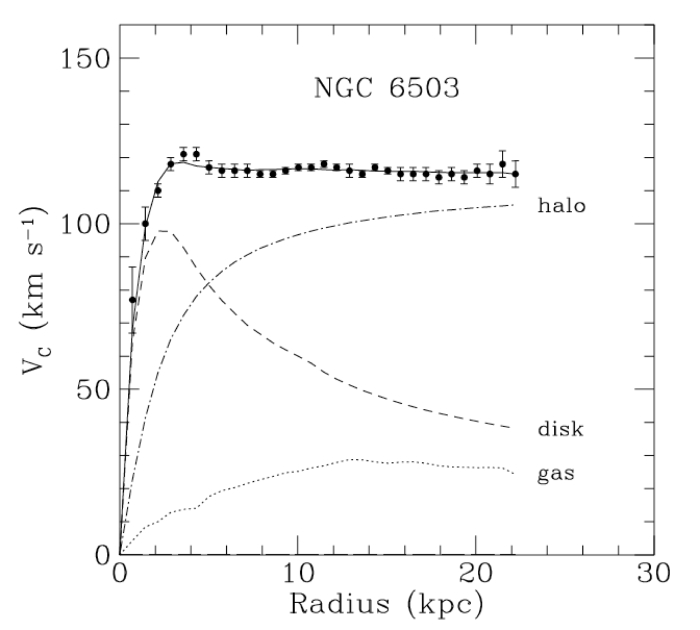
\includegraphics[width=0.4\linewidth]{plots/DarkMatter/RotationCurve_NGC6503.png}
\caption[The rotation curve of galaxy NGC~6503]{The measured rotation curve of the galaxy NGC~6503 from Ref.~\cite{RotationCurves_Begeman}, also showing the rotational-velocity profiles for the individual components of gas, stars, and the dark matter halo.}
\label{figRotationCurve}
%\end{figure}
\end{floatingfigure}

\begin{equation}
\label{eqVirialMass}
M_{\mathrm{tot}} \simeq \frac{2 \cdot R_{\mathrm{tot}} \cdot v^{2}}{G}.
\end{equation}

The amount of luminous matter is indicated by the luminosity of the galaxies. The measurements showed a deficit of luminous matter with respect to the mass of the cluster, which indicates the presence of large quantities ($>$90\%) of invisible mass, which is is revealed only by its gravitational interaction. The initial observation has been confirmed by a survey of the virial masses for 89 galaxy clusters, indicating the average mass-to-light ratio of 230$-$250~\cite{VirialMasses}.

Another evidence for the presence of dark matter has been found at galactic scale in the analysis of {\it rotation curves} of stars and gas~\cite{RotationCurves_Rubin} in disk galaxies, by measuring the redshift as a function of the distance $R$ to the galactic center. The light from the stars can be used for this purpose, but a clearer measurement has been performed by observing the emission of neutral hydrogen~\cite{RotationCurves_Begeman}, as its cloud typically extends far beyond the visible disk of stars, and hence can probe a larger region than the stars themselves. Since the majority of the luminous mass is located at the galactic center, it was expected that the motion of stars can be predicted by Newtonian dynamics, and the circular velocity should scale as $R^{-1/2}$. However, this is not the case for most galaxies, as shown in Fig.~\ref{figRotationCurve} by an example of galaxy NGC~6503~\cite{RotationCurves_Begeman}. The rotation curves of spiral galaxies are flat, while the stellar density falls off exponentially at large radii and hence cannot account for the observation. 
This indicates the existence of non-luminous matter superimposed upon the luminous disk. The rotation of the galaxies can be explained by introducing a dark matter halo with a mass density proportional to $R^{-2}$. The sum of the contributions from the visible matter in the disk and from the hydrogen gas, and dark matter in the halo reproduces the observed rotation curve.

Further evidence for invisible matter on the scale of galactic clusters is the phenomenon of {\it gravitational lensing}~\cite{GravitationalLensing_Review}, where a galaxy cluster acts as a lens for the light emitted from a more distant galaxy with high surface brightness, bending it with its gravitational field (see Fig.~\ref{figGravitationalLensing}) and resulting in multiple images of the background galaxy. Measurements of the light deflection provide a possibility to determine the mass of the galaxy cluster. This value is then compared to the luminous mass, which is calculated based on the X-ray luminosity. The mass-to-light ratio measured with this method~\cite{GravitationalLensing_Observation} confirms the results of the velocity dispersion measurements, pointing at the presence of a large fraction of non-luminous non-baryonic matter (dark matter). Additionally, it indicates the existence of non-luminous, but baryonic, component in the form of X-ray emitting plasma, which exceeds the mass of luminous matter by a factor of $\sim$6~\cite{GravitationalLensing_XrayPlasma}.

One of the strongest evidences for the existence of dark matter has been obtained by observing collisions of galaxy clusters~\cite{GravitationalLensing_BulletCluster, GravitationalLensing_Abell, GravitationalLensing_MACS1, GravitationalLensing_MACS2}. The diffuse clouds of the hot X-ray emitting intracluster plasma and interact electromagnetically, slowing down in the collision process, while the stars simply pass by one another without large disturbance. Since conglomerations of dark matter experience only gravitational interactions, they will also pass through one another, and hence exhibit very different dynamics during the collision compared to the hot interstellar gas. An example of such collision for Bullet cluster (1E0657-558)~\cite{GravitationalLensing_BulletCluster} is shown in Fig.~\ref{figGravitationalLensing_2}. The extent of cluster plasma, determined from X-ray emission, is shown in pink, and the distribution of the mass of the cluster, measured by gravitational lensing, is indicated in blue. The clouds of hot gas (baryonic matter) have been stripped away from their parent clusters, while the dominant mass is laterally displaced from the baryonic matter, thus showing a discrepancy in the strength of the gravitational force, consistent with the expectation of collisionless dark matter.

%\begin{floatingfigure}[r]{0.3\textwidth}
\begin{figure}[!h]
\centering
\subfigure[]{
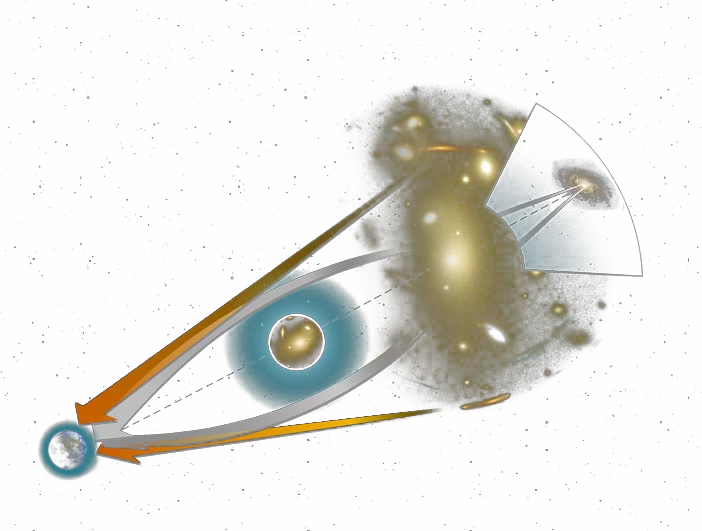
\includegraphics[height=0.325\linewidth]{plots/DarkMatter/GravitationalLensingNASA_white.png}
\label{figGravitationalLensing_1}}
\subfigure[]{
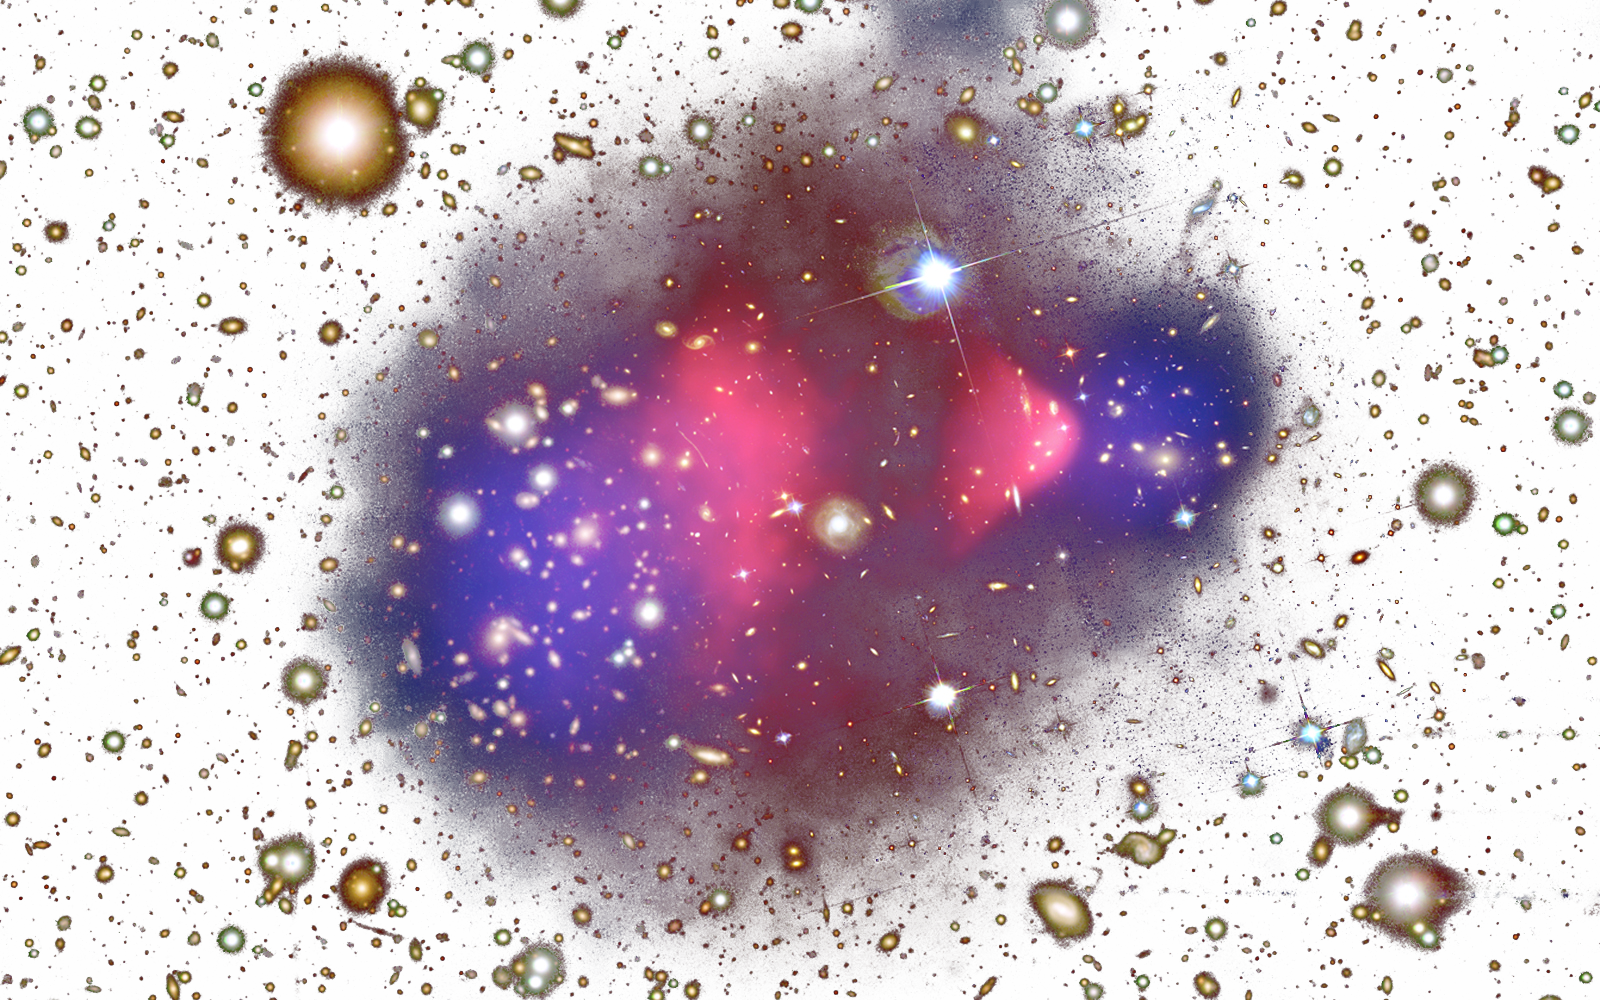
\includegraphics[height=0.325\linewidth]{plots/DarkMatter/BulletCluster_white.png}
\label{figGravitationalLensing_2}}
\caption[The gravitational lensing effect and the Bullet cluster with two colliding galaxy clusters]{(a) - the gravitational lensing effect: the galaxy cluster in the front acts as a strong gravitational lens for a distant galaxy behind with high surface brightness.  (b) - the Bullet cluster with two colliding galaxy clusters. The majority of the baryonic mass is located in the intracluster plasma, shown in pink, and the dominant cluster mass is shown in blue. Their displacement from one another can be explained by dark matter. Figures from Ref.~\cite{NASA}.}
\label{figGravitationalLensing}
\end{figure}
%\end{floatingfigure}

Evidence for dark matter on a universal scale is provided by the measurements of the cosmic microwave background (CMB), photons at microwave wavelengths, which exists as a consequence of the Big Bang. The temperature spectrum of CMB gives detailed information about the energy density at the time of photon decoupling. The data from Wilkinson Microwave Anisotropy Probe (WMAP)~\cite{WMAP_5year, WMAP_7year} has been used to measure the total matter and energy density in the universe ($\Omega_{tot}$ = 1.02$\pm$0.02), the total matter density ($\Omega_{m}$ = 0.266$\pm$0.029), and the density of baryonic matter ($\Omega_{b} = $0.0449$\pm$0.0028). This baryonic matter contributes only about 17\% of the matter density in the universe, and its density matches with the one from luminous mass measurements.

A standard cosmological model ($\Lambda$CDM) has been developed by combining the measurements of astrophysical systems at sizes ranging from galactic to universal scales. In this model, 4.6\% of the universe consists of atoms, the building blocks of stars and planets, 23\% is composed of non-baryonic dark matter that does not emit or absorb light, and so far is detected only indirectly by gravitational forces, as detailed above.  The remaining 72\% is an unknown component called dark energy that is responsible for the present-day acceleration of the expansion of the Universe~\cite{DarkEnergy}.

%On a universal scale 


